% This is LLNCS.DEM the demonstration file of
% the LaTeX macro package from Springer-Verlag
% for Lecture Notes in Computer Science,
% version 2.4 for LaTeX2e as of 16. April 2010
%
% !TeX spellcheck = en_GB
\documentclass{llncs}
%
\usepackage{makeidx}  % allows for indexgeneration

%custom
\usepackage{glossaries}
\usepackage{graphicx}
\usepackage[utf8]{inputenc}
\usepackage{comment}

\newacronym{atam}{ATAM}{architecture trade-off analysis method}
\newacronym{htn}{HTN}{Hierachical Task Network}
\newacronym{hipop}{HiPoP}{Hierarchical Partial-Order Planning}
\newacronym{dl}{DL}{Description logic}
\newacronym{kb}{KB}{knowledge base}
\newacronym{BDI}{BDI}{Belief-desire-intention}
\newacronym{pa}{PA}{planning agent}
\newacronym{ea}{EA-BDI}{service provider expert agent}
\newacronym{fifo}{FIFO}{First-in-first-out}
\newacronym{ws}{WS}{web service}
\newacronym{csp}{CSP}{constraint satisfaction problem}
\newacronym{fol}{FOL}{first order logic}
\newacronym{owl}{OWL}{Web Ontology Language}
\newacronym{rdf}{RDF}{Resource Description Framework}
\newacronym{rdfs}{RDFS}{Resource Description Framework Schema}
\newacronym{obda}{OBDA}{Ontology-Based Data Access}
\newacronym{mas}{MAS}{Multi-agent system}
\newacronym{FIPA}{FIPA}{Foundation for Intelligent Physical Agents}
\newacronym{acl}{ACL}{Agent Communication Language}
\newacronym{kqml}{KQML}{Knowledge Query and Manipulation Language}
\newacronym{kif}{KIF}{Knowledge Interchange Format}
\newacronym{cc}{C\&C}{Component and Connector}
\newacronym{soa}{SOA}{Service Oriented Architecture}
\newacronym{rest}{REST}{Representational state transfer}
\newacronym{aoa}{AOA}{Agent Oriented Architecture}
\newacronym{bnf}{BNF}{Backus-Naur Form grammar}
\newacronym{ai}{AI}{Artificial Inteligence}
\newacronym{jvm}{JVM}{Java virtual machine}
\newacronym{rae}{RAE}{Refinement acting engine}
\newacronym{ipoe}{IPOE}{Input-Preconditions-Output-Effect}
\newacronym{ATAM}{ATAM}{Architecture Tradeoff Analysis Method}
\newacronym{SP}{SP}{service provider}
\newacronym{SAAM}{SAAM}{Software Architecture Analysis Method}


%
\begin{document}
%
\frontmatter          % for the preliminaries
%
\pagestyle{headings}  % switches on printing of running heads
\addtocmark{Belief desire intention architecture for virtual intelligent agents: travel assistant case study} % additional mark in the TOC
%
\mainmatter              % start of the contributions

\title{An approach to designing Belief-Desire-Intention based virtual agents for travel assistance}

\author{Arūnas Miliauskas \and
Dalė Dzemydienė}

\institute{Vilnius University, Institute of Data Science and Digital Technologies, Vilnius, Lithuania}

\maketitle
%
% Modify the bibliography environment to call for the author-year
% system. This is done normally with the citeauthoryear option
% for a particular contribution.
%
\begin{abstract}
	The aim of this research is to propose a \gls{BDI} architecture-based approach for a virtual agent design. A presented case of a chatbot assistant in a travel domain demonstrates the necessity of the \gls{BDI} architecture modification. The approach is taken for multiple  \gls{BDI} agent instances with a shared external knowledge base. The proposed architecture is evaluated with a simplified version of \gls{ATAM}. The evaluation shows that the architecture supports provided modifiability, performance scenarios, but introduces several risks.
%The abstract should summarize the contents of the paper using at least 70 and at most 150 words. It will be set in 9-point font size and be inset 1.0 cm from the right and left margins. There will be two blank lines before and after the Abstract. \dots
\keywords{Software architecture, Belief-Desire-Intention architecture, Distributed databases, Travel assistance}
\end{abstract}
\section{Introduction}
 
Our object of research is an assistant-broker agent that supports end-user in activities like travel planning, meeting arrangement. The agent could, using provided web services, complete main action behalf of user. 

This topic is not new. %Intelligent agents are often envisioned as important component for semantic web that uses information provided by web services. 
The \gls{FIPA} organization provided personal travel assistance specification \cite{fipa000132000fipa}. It provides a scenario and an architecture of a potential distributed agent based system, where an end-user can get assistance and support in a trip planning. That show quite big expectations towards intelligent agents for the semantic web. However, we still don't see today widespread intelligent agents like the personal travel assistant presented by \gls{FIPA}.

\begin{comment}
However, most of agent architectures applications we proposed for robotic field. We see such differences from application of agents in robotic field from building semantic web based information agents (term \emph{information agent} is defined \cite{wooldridge1995intelligent}):
\begin{enumerate}
	%\item a robotic application has limited resources, whereas web agent have access to cloud service and can increase its storage and computational resource on demand if is designed to do so
	\item web based agent may obtain big amount of information, therefore scalable approaches for agent knowledge base management may be needed;
	\item new sources of information can be added later and data model should be adaptable enough.
	%\item due to limited resources of autonomous robot each action has to be interruptible, what is not so important in web agent
\end{enumerate}
\end{comment}


%\section{Related works}
 %\section{Research methodology}
\gls{BDI} \cite{rao1995bdi} is a well know agent architecture. It is based on main concepts  \emph{Belief}, \emph{Desire} and \emph{Intention}, which ought to have an explicit representation in this type architecture. 

In this research, our goal is to analyse \gls{BDI} architecture application possibilities for building a virtual agent - travel assistant chatbot.

We  use the framework \cite{wieringa2014design} for design science. The result of a design is an artifact, based on actual or hypothetical stakeholder goals which are represented in Section \ref{sec:social-context}. 

\begin{comment}
The artifact is evaluated using adapted version of \gls{atam}. There are many proposal for software architecture evaluation based on quality requirements \cite{babar2004comparison}. The \gls{atam} \cite{kazman2000} has been widely adopted in the software industry and has many published cases. However, we simplify it to our research. We take our hypothetical business drivers, generate scenarios for important quality attributes and probe the architecture using scenario walk-through technique. Based on that, sensitivity points, trade-offs and risks are identified. % This technique was used in \gls{SAAM} \cite{kazman94saam}, the predecessor of \gls{ATAM}.
\end{comment}

The architecture is defined using the Views and Beyond approach \cite{bachmann2010documenting}. It is arranged in views, where architecturally important structures are described from a particular viewpoint.

We extend architecture descriptions with a decision view \cite{kruchten2009decision}. It contains architectural decisions and their relations, which are based on ontology of architectural decisions \cite{kruchten2004Ontology}.

The remainder of this paper is structured as follows. Section \ref{sec:architecture} describes the architecture and it's context. Section \ref{sec:evaluation} contains evaluation of the architecture. Final conclusions are drawn in Section \ref{sec:conclusions}

% Design view
%ISO/IEC/IEEE 42010 addresses the areas of recording architecture decisions and architecture rationale as part of an architecture description, specifying general requirements for decision documentation, but not particular mechanisms 

\section{Assistant Agent Architecture}
\label{sec:architecture}
The architecture specification starts with business drivers presentation in Section \ref{sec:social-context}. Then, based on \cite{bachmann2010documenting}, views are presented. We introduce a separate context view in Section \ref{sec:context-view}. Main views, related to structure of the target system, are Module Decomposition view and \gls{cc} hybrid view. Former presents overall structure of system, whereas latter describes a structure for one of main elements. These views are presented in Sections \ref{sec:module-decomposition} and \ref{sec:hybrid-view}, respectively. We add a decision view in Section \ref{sec:decisionview} to demonstrate relations between architectural decisions and drivers.
 
\subsection{Business drivers}
\label{sec:social-context}
Main drivers represents expected qualities, constraints and assumptions: 
\begin{itemize}
	\item \emph{D1. Big amount of information}. This assumption is related to amount of information that can be obtained from \gls{SP} services. A property "big" is vague, therefore we use an example from the travel domain. Here information is about potential flights, hotels, car hire service and their prices. We expect the system to be able collect this data from \gls{SP} services and provide, apart precise date search, an exploration for best prices. An amount of information that must accessed, handled by the system is referred as "big".
	\item \emph{D2. Varying change rate for information}. Some information in travel domain is static and some changes often. For example we see frequent flight prices changes and stable flight schedule.
	\item \emph{D3. Response latency} is taken from current \gls{SP} services in the travel domain. We have observed that response latency usually is bigger than 1 second and less than 1 minute. The agent should have same response latency values.
	\item \emph{D4. Chatbot}. This requires that assistant should be a chatbot.
	\item \emph{D5. Non-critical availability}, since user could accomplish task "old way".
	\item \emph{D6. Modifiability important}. This means emphasis on modifiability since adding new service providers may require a modification.	
	\item \emph{D7. No standartized services}. This assumption states that there should not be any expectations for standardized \gls{SP} web services. The system must operate with existing services and this potentially requires an adaptation for each service provider.
	\item \emph{D8. SP uses REST}. This is an assumption that \gls{rest} architectural style \cite{fielding2000architectural} is used by \gls{SP}s.
\end{itemize}
All drivers are used in Section \ref{sec:decisionview} and visually represented in Fig. \ref{fig:decisions}

\subsection{Context view}
\label{sec:context-view}
\subsubsection{Primary presentation.} Diagram is presented in Fig. \ref{fig:maincontext}. It contains a context and main parts (internal structure).  Here we define only the context and skip the internal structure.
\begin{figure}[t]
	\centering
	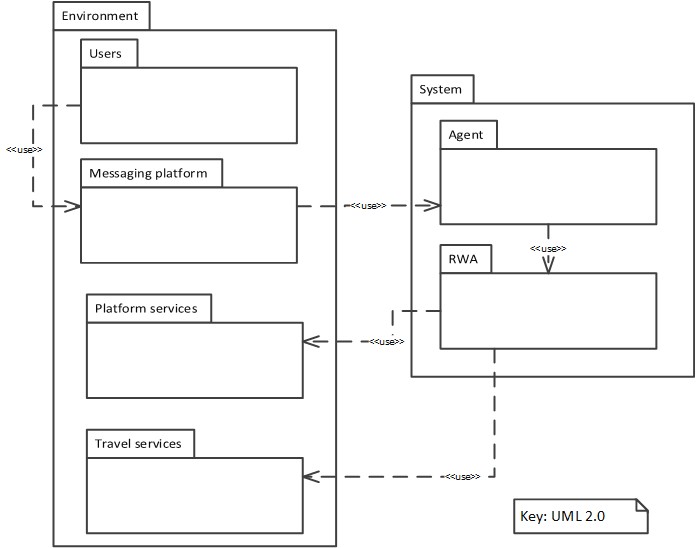
\includegraphics[width=\linewidth]{Images/BDIDecomposition.png}
	\caption{Main modules and context}	
	\label{fig:maincontext}
\end{figure}
\subsubsection{Element catalog.}
% kur dėti tokius servisus kaip billing'o servisas?
% ir toks skirstymas turi vėliau turėti prasmės. Vėlesnėse diagramose platform services neišskiriami o naudojami travel services
% jei tai pagal business domain analysis kaip FIPA tai reiktų gal nuorodos į tą metodologiją.
System is envisioned to be placed in environment that consists of: \begin{enumerate}
	\item \emph{users}, which are end users that are expected to use system. However they don't use directly the system, but communicate using \emph{communication platform}.
	\item \emph{communication platform} is a medium that end-user uses for communication. It can be a platform like Skype, Facebook messenger, Slack and others. 
	\item \emph{platform services}, which are cloud based platform services that provide storage, computing services.
	\item \emph{travel services}, which represents services providers like airlines, hotels etc.
	\item \emph{system} - the proposed system, which will be refined to details in other views. 
\end{enumerate}


\begin{comment}
\subsubsection{Rationale}
The main rationale for splitting an environment is based on a position of brokerage in travel business domain, where broker acts as intermediary between users and travel service providers. Since there is a requirement to use cloud service for building and running system, an additional package that describes platform service is introduced. To simplify diagram, packages are not refined in details.

\subsubsection{Variability}
Despite that our research is focused on building chatbots, this model is compatible with other ways for using by end-users the system. The \emph{communication platform} encapsulates communication methods with the end-user. For example, the \emph{communication platform} might support voice based communication.

Since there exists \emph{uses} relation from system to \emph{Platform services} and \emph{Travel service}, at this abstraction level, there are many ways how usage can be carried out.
\end{comment}

\subsection{Module decomposition view: System}
\label{sec:module-decomposition}
\subsubsection{Primary presentation.} The primary presentation diagram is presented in Fig. \ref{fig:maincontext}

\subsubsection{Element catalog.} The system is decomposed to modules:
\begin{itemize}
	\item \emph{Agent} that encapsulates all intelligent behaviour,
	\item \emph{RWA} (stands for real world adapter) - an intermediary between \emph{Agent} and \gls{SP} web services.
\end{itemize}
\subsubsection{Design rationale.} The decomposition is result of the architectural decision \emph{AD3. Decompose 2 RWA \& agent} and is explained in Section \ref{sec:decisionview}. Another reason is that we want to encapsulate issues related to agent interoperation with environment into a separate module and then focus mainly on the agent part.

\begin{comment}
The main reason of following decomposition is agents for achieving following qualities \begin{itemize}
	\item interoperability - in order agent to work with existing services new element is added \emph{RWA} which contains all necessary adaptation and data transformation to enable operations with existing services.
	\item  modifiability - is handled in both elements \emph{agent core} and \emph{RWA}, but in different ways. More details is discussed with presentation of their internal structure bellow %TODO papildyti %When new service providers are added.
\end{itemize}
 Separate \emph{RWA} element which contain modification required to connect to new or changed services.

\end{comment}

\subsection{Hybrid \gls{cc} view and module decomposition view: Agent}
\label{sec:hybrid-view}

A \gls{cc} communicating processes view emphasizes concurrently running units and their interactions. Concurrently running units can be processes or threads. They interact by communication or synchronization and this interaction is represented using connectors. %Also important is data stores that are accessed by concurrently running units. However, here we focus and present in view only those that are accessed by concurrent units. 
% agent can be similar to active and passive objects(or active passive classes)
\subsubsection{Primary presentation.}
The primary presentation diagram is presented in Fig. \ref{fig:agent}. Here \gls{cc} style is mixed with module style. At highest level, the components are provided. However, an \emph{agent} component is further decomposed to details, where his internal structure is defined in a module view. The reason for this representation is desire to represent all \gls{BDI} elements in single diagram.
\begin{figure}[t]
	\centering
	\includegraphics[width=\linewidth]{Images/agent.png}
	\caption{Agent module}	
	\label{fig:agent}
\end{figure}
\subsubsection{Element catalog.}
 \emph{Agent} module here is implemented by main 2 agent components: \begin{itemize}
	\item \emph{ConversationalAgent}, which is responsible for maintaining conversation with end-user. It receives end-user messages identifies intentions and translates them to an agent communication language.
	\item \emph{AssistantAgent}, which responsible for an assistance process. This component receives messages from \emph{ConversationalAgent}, percepts environment and acts in it.
\end{itemize}
\emph{KB} represents a \gls{kb} of the target system, which is implemented externally (from the \emph{agent} component perspective).
\emph{AtomicActionService} represent a component that implements an atomic action. Each atomic action is implemented by a separate component, which implements \emph{IAtomicAction} interface.
\emph{Agent} is decomposed into modules: \begin{itemize}
	\item \emph{ExternalCommunication} - module responsible for communication external entities. It exposes IMessages interface for receiving messages and uses provided IMessagesResponses to send responses.
	\item \emph{Acting} module that is responsible for an intended action execution. It has link with \emph{ExternalCommunication}, because sending a response message is also considered as act. It uses an IAtomicAction interface provided by \emph{AtomicActionService}, to execute an action in the environment. Action results are sent to \emph{Perception}. 
	\item \emph{Perception} module is responsible for sensing the environment. Since in the travel domain sensing is possible by querying services, which is treated as acting, this module receives data from \emph{Acting} module.
	\item \emph{DecisionMaking}, which further is decomposed: \begin{itemize}
		\item \emph{Interpreter}, which is responsible for sensing, choosing candidate methods and acting based on selected methods. It interprets statements in a method's body and executes them (acts).
		\item \emph{Agenda}, which represent agent active intentions (in \gls{BDI} terms) in a \emph{IntentionGraph}.  %TODO: reiktu tikslinti bet panasu nespesiu
		\item \emph{MethodLibrary}, which represents agent desires (in \gls{BDI} terms) and contains (in a method body) "recipies" how desires could be achieved.
	\end{itemize}
\end{itemize}
\subsubsection{Design rationale.} Since all design decisions are defined in Section \ref{sec:decisionview}, here we relate the presented structure with these decisions. Components \emph{ConversationalAgent} and  \emph{AssistantAgent} are introduced by the decision \emph{AD5. Split conversation \& assistance}. \emph{AD7. BDI} defines structure of  \emph{AssistantAgent}. However since this decision doesn't comply with requirements other decisions required that shape the presented structure:
\begin{itemize}
	\item \emph{AD8. Shared KB agents} introduces a component \emph{KB} outside \emph{AssistantAgent} with defined interfaces.
	\item \emph{AD13. Intention stack processing} introduces \emph{IntentionGraph} and modifies \emph{Interpreter} (changes not visible from this view).
	\item \emph{AD14. Acting/sensing} changes are that \emph{Perception} module is connected to environment only via \emph{Acting} module.
	
\end{itemize}

% AD9? A10?




%To avoid wishful thinking
\subsection{Decision view}
\label{sec:decisionview}
We present main architectural decisions and relations between them and business drivers.
\subsubsection{Primary presentation.}
Primary presentation, in Fig. \ref{fig:decisions}, consists of main requirements (represented by rectangles), architectural decisions (represented by diamond shapes) and their relations. %When possible, we use same relationships for connecting requirements with architectural decisions as between architectural decisions. 
It is simplified version leaving only decisions that are necessary for explanation and reasoning. Each decision is either in a decided or rejected/obsolesced state. Former ones are represented by filled shape and have an architecture decision identifier, whether latter ones don't have any identifiers and have corresponding shapes not filled.
\begin{figure}[t]
	\centering
	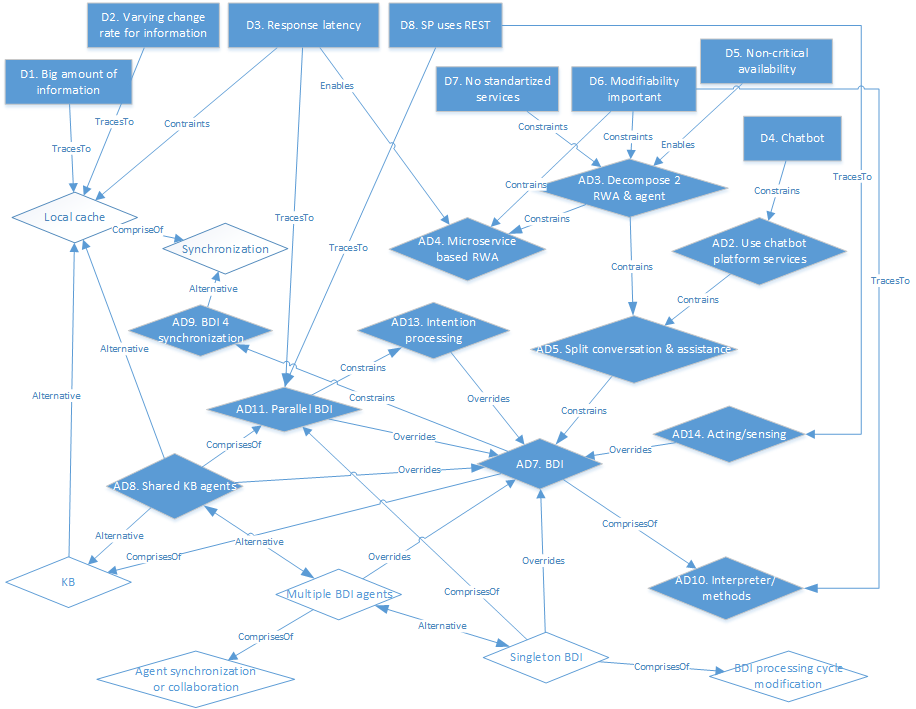
\includegraphics[width=\linewidth]{Images/decisions.png}
	\caption{Decision dependencies}	
	\label{fig:decisions}
\end{figure}
\subsubsection{Element catalog}
contains decisions: \begin{itemize}
	\item \emph{Local cache} it means introducing data redundancy. It is an existence decision \cite{kruchten2004Ontology}, stating that the element should appear is the system.  However, it is abstract and doesn't bring any implementation details.  It is based on a business driver D3 for achieving required performance in context of other drivers D2, D1. This decision doesn't forbids, real-time access to \gls{SP}s service for responding for end-user requests. Moreover, drivers D2, D1 suggest balancing between using cached information and real-time \gls{SP} services access. Also this decision brings out a sub-decision to have data \emph{synchronization}. 
	\item \emph{Synchronization} decision means that should be a mechanism for data synchronization, without explicitly stating how it is carried out.
	\item \emph{AD2. Use chatbot platform services} is decision to use current cloud services providers as IBM Watson cloud, Microsoft Azure and others.
	\item \emph{AD3. Partition modules} represents decision splitting responsibilities into modules. It is intended to support modifiability requirement (D6). The other driver D5 enables this decisions. The decision is decomposed to sub-decisions that are related to constituent parts resulting in this split: \emph{AD5. Split conversation and assistance} and \emph{AD4. RWA}.
	\item \emph{AD4 RWA} means introducing a module, to hide \gls{SP} services.
	\item \emph{AD5. Split conversation and assistance} is a decision to split responsibilities between assistance and conversation modules. Former module is responsible for whole assistance process and the latter one is for the conversation (recognizing end-user intents).   % TODO: kodel?
	\item  \emph{AD7. BDI}  is the decision to use a \gls{BDI} model for the assistance module. That brings out several decisions: \emph{KB}, \emph{AD10. Interpreter/methods}. However, it doesn't comply with performance requirements and modifications are needed. Additional decisions are introduced that override some properties of the \gls{BDI} model.
	\item \emph{KB} is an existence architectural decision introduced by \emph{AD7. BDI} decision. This decision is alternative to the \emph{Local cache} decision.
	\item \emph{AD10. Interpreter/methods} is introduced by \emph{AD7. BDI} decision. It defines that architecture should contain interpreter and library of methods, written in specific language. 
	\item \emph{AD8. Shared KB agents} is a decision to implement multiple agents based on a single shared \gls{kb}. Therefore, it overrides the initial decision (\emph{AD7. BDI}) and makes the \emph{KB} decision obsolete (is alternative). We also describe some alternatives:
	\begin{itemize}
		\item The use of singleton \gls{BDI} agent responding multiple user requests - \emph{Singleton BDI}. This requires significant modifications of the \gls{BDI} agent. One of them is an introduction of concurrency. Another is a \gls{BDI} processing cycle adaptation to handle multiple end-users requests in parallel. This alternative requires introducing parallel execution of actions \emph{AD11. Parallel BDI}
		\item Using multiple \gls{BDI} agent instances where each has a separate \gls{kb} - \emph{Multiple BDI agents}. This requires an agent knowledge synchronization, sharing mechanism or multi-agent collaboration for single end-user request.
	\end{itemize} 
	We see that described alternatives are more complex and requires more effort, than selected \emph{AD8. Shared KB agents}.
	\item \emph{AD9. BDI for synchronization}, by taking decision \emph{AD7. BDI}, this enables use \gls{BDI} agent for synchronization, what is an detailed alternative to abstract \emph{Synchronization} decision.
	\item \emph{AD11. Parallel BDI} is a decision to introduce the ability to execute simultaneously multiple information gathering (sensing) actions. The  agent is expected to collect and aggregate many \gls{SP}s information. We can not make assumption about a sufficient \gls{SP} web service response latency. This leads to a decision querying these services in parallel and mixing results with the cached information. However, this property decision doesn't state how this is implemented.
	\item \emph{AD13. Intention processing} refines the decision \emph{AD11. Parallel BDI} with implementation details. It is about changes in \gls{BDI} agenda part that intentions should be organized using a graph instead of a stack structure. The \gls{BDI} processing cycle should also be modified to manage multiple active intentions in the graph.
	\item \emph{AD14. Acting/sensing} is decision to relating acting and sensing. Since \gls{SP} provide information using web services, sensing is a result of acting.
\end{itemize}



\begin{comment}


\subsubsection{Reasoning} %todo. pakeisti  
%Reasioning view visually indicates
This view visually indicates \begin{itemize}
	\item changes need to \gls{bdi} model in this setting - it is decisions that overrides decision \gls{bdi}
	\item how initial decision \emph{LocalCache} and \emph{PartitionModule} relates to subsequent decisions.
\end{itemize} 
This represents use cases: "Evaluate impact of an architectural decision" and "Detect patterns of architectural decision dependencies" \cite{ven2006using}
\end{comment}

\begin{comment}
\section{Architecture evaluation}
\label{sec:evaluation}

The architecture evaluation is based on simplified version of \gls{atam} \cite{kazman2000} . Here, there are scenarios elicited and the architecture is probed using a scenario walk-through technique. Based on that, sensitivity points, trade-offs and risks are identified and grouped into main risk themes. 

Scenarios are presented in Section \ref{sec:scenarios}. The scenario-based walk-through is described in Section \ref{sec:architecture-analysis}, where risks, trade-offs and sensitivities are identified. Section \ref{sec:architecture-results} presents results, where main risks themes are mapped with decision view elements.

\subsection{Scenarios}
\label{sec:scenarios}
The provided architecture is analysed with scenarios. All scenarios belong to a particular quality attribute and form leaves in a utility tree. A tabular  form of the utility tree is presented in Table \ref{tbl:utilitytree}. We use a shortened scenario version \cite{bass2012softwareArchitecture} with stimulus, environment and response.
\begin{table}
	\setlength{\tabcolsep}{0.3em}	
	\caption{Utility tree}
	\label{tbl:utilitytree}
	\begin{center}
		\begin{tabular}{c | p{2.2cm} | c}
			\hline			
			Id &
			Quality \newline attribute&	Scenario \\		
			\hline

			Pt1 &
			Modifiability - \newline Portability  &
			\begin{tabular}{r p{7cm} }
				(Stimulus) & \gls{SP} changes a service. Syntactical changes of provided data \\
				(Environment) & At runtime \\
				(Response) & Affected elements in the architecture are identified and changes are implemented
			\end{tabular}
			\\ \hline
			Pt2 &
			Modifiability - \newline Portability  &
			\begin{tabular}{r p{7cm} }
				(Stimulus) & \gls{SP} changes a service. Semantic changes of provided data \\
				(Environment) & At runtime \\
				(Response) & Affected elements in the architecture are identified and changes are implemented
			\end{tabular}
			\\ \hline
			Md1 &
			Modifiability  &
			\begin{tabular}{r p{7cm} }
				(Stimulus) &  A change request arrives, for extending or adding new functionality based on the same environment\\
				(Environment) & At development time \\
				(Response) & Locations to be changed are identified, changes are implemented, tested and deployed.
			\end{tabular}
			\\ \hline			
			Md2 &
			Modifiability  &
			\begin{tabular}{r p{7cm} }
				(Stimulus) & Change request arrives, for extending or adding new functionality that requires changing interoperation with the environment\\
				(Environment) & At development time \\
				(Response) & Locations to be changed are identified, changes implemented, tested and deployed
			\end{tabular}
			\\ \hline
			Pf1 & 
			Performance  &
			\begin{tabular}{r p{7cm} }
				(Stimulus) & End-user requests information\\
				(Environment) & At runtime \\
				(Response) & \gls{SP} services are requested, their result is transformed, mapped with local information and returned.
			\end{tabular}
			\\ \hline
			Pf2 &
			Performance  &
			\begin{tabular}{r p{7cm} }
				(Stimulus) & Sporadic arrival of user requests\\
				(Environment) & At runtime  \\
				(Response) & Each user request handled concurrently.
			\end{tabular}
			\\ \hline
			Pf3 &
			Performance  &
			\begin{tabular}{r p{7cm} }
				(Stimulus) & New data or new methods added\\
				(Environment) & At runtime or development time \\
				(Response) & Ability to handle requests efficiently in terms of the latency elasticity to the size of stored information.
			\end{tabular}
			\\ \hline
		\end{tabular}
	\end{center}
\end{table}



%\section{Assistant Agent Architecture. KISS approach}
%\label{kiss-approach}
 \subsection{Analysis}
 \label{sec:architecture-analysis}
We analyse the architecture using the quality attribute tree. The analysis is structured around quality attributes. %Each risks, tradeoff or sensitivity point is given an identifier and this identifier is used in place where it is found.
%\subsection{Reasoning about quality attributes}
\subsubsection{Modifiability}
\paragraph{Pt1} The architecture supports this scenario by introducing \emph{RWA}. Since changes are related to data syntax, these changes are accommodated by creating needed transformations in \emph{RWA}. However, adding layers and implementing them as web services might affect other qualities like performance. This is identified as a trade-off T1.
\paragraph{Pt2} In this scenario \gls{SP} deploys new services which are semantically un-interoperable. By term semantically un-interoperable, we mean that either changed interaction protocol or services data model is incompatible with our system model. 

In this scenario, there are expected changes in modules: \emph{RWA}, \emph{AtomicActionService}, \emph{MethodLibrary} (by modifying, adding, removing instances of type \emph{Method}). Here, a introduction of \emph{RWA} layer may negatively affects this scenario, since the number of affected modules are increased. This is a sensitivity point S10.

Changes in the agent part is supported by a \gls{BDI} architecture style. It introduces an \emph{Interpreter} pattern, which is an architectural decision of \emph{Increasing abstraction level} \cite{bachmann2007modifiability}. The application of this pattern is expected to reduce cost of modifying a responsibility. However, the \gls{BDI} architecture allows multiple methods for accomplishing same task and method selection can be non-deterministic. This complexity negative affects testability and is tradeoff T2.
\paragraph{Md1} This scenario is about modifying functionality without changing any interaction with the environment. Therefore modules like \emph{RWA} should not be affected. Subject for modifications are: \emph{ConversationalAgent}, \emph{MethodLibrary} (instances of \emph{Method}) and potentially \emph{AtomicAction}. Last is added to list, since several \gls{SP} services can be encapsulated by one atomic action and this might appear inconsistent with new requirements. At this level of architecture, there is no distinct separation between \emph{AssistantAgent} and \emph{AtomicActionService} modules. Main idea that atomic actions should be composable in agent methods and should not change unless environment changes. The actions should be designed in later stages (depending on a approach): during domain analysis and design or service oriented analysis and design \cite{ErlSoa2016}. Since decision of defining boundary between methods and atomic is postponed to later stages it is identified as risk R9.
\paragraph{Md2} In this scenario requirements can be fulfilled only by changing interaction with the environment. Therefore changes are expected in  \emph{ConversationalAgent}, \emph{MethodLibrary} (instances of \emph{Method}), \emph{AtomicActionService} and \emph{RWA}. This scenario, in term of effect to the architecture, is same to scenario Pt1.

\subsubsection{Performance}
\paragraph{Pf1} A response measure for this scenario is latency. 
Introducing redundancy by adding \emph{KB} supports performance, but adds need for synchronization, what negative impacts testability (tradeoff T3).

Adding layers, which are implemented as microservices, negative affects latency (tradeoff T1). 

Concurrency introduction in a \gls{BDI} model reduce latency, however might add contention for shared resources like \emph{KB} (sensitivity point S4). The model is based on continuous cycle, where for event applicable methods are filtered. This is sensitive to amount of events introduced by multiple agents (sensitivity point S7) and to growth of data in \emph{KB} and \emph{MethodsLibrary} (S8) 

Using the \gls{BDI} model with external \gls{kb} might negative affect latency (however may increase scalability, which performance elasticity to load) and gives a sensitivity point S5. 
\paragraph{Pf2} The architecture supports scenario by instantiating new \emph{AssistantAgent} and \emph{ConversationalAgent} pair for each end-user. However adding more agents, which are bound to same shared resource \gls{kb} is sensitivity point related to performance (S6).
\paragraph{Pf3} The system is sensitive to the size of \emph{MethodsLibrary} or \emph{KB}. Therefore a sensitivity point S8 is added.

\subsubsection{Sensitivies, tradeoffs and risks.}
Summary of risks, sensitivities and tradeoffs is presented in Table \ref{tbl:risks}. In original \gls{ATAM} each tradeoff should be categorized as a risk or non-risk. Here we take all sensitivities and tradeoffs as potential risks. All risks are grouped in risk themes. An additional impact measure is added to risk theme. High impact means that additional decisions required for mitigating these risks in this theme. %todo kodel reiktu. 
Low impact means that these risks should be taken into account and monitored, whether some deviations might occur in case of changing requirements.
\begin{table}	
	\setlength{\tabcolsep}{0.5em}
	\caption{Sensitivies, tradeoffs  and risks }
	\label{tbl:risks}
	\begin{center}
		\begin{tabular}{  l | p{23em} | l | p{6em} }
			\hline			
			Id &
			Description &
			Impact &
			Risk themes
			 \\		
			\hline
			T1 & 
			Adding layers, implemented as web services, negatively affects performance (latency), testability and availability. 
			%Also it can negatively affect modifiability when changes affects all layers  
			& 
			Low
			&	
		Microservices chain tradeoff \newline Testability
			\\ \hline
			T2 & 
			Adding interpreter affect testability, since \gls{BDI} method selection might include some nondeterminism  & High &
			Testability
			\\ \hline
			T3 &
			The redundancy introduction (by adding a local \gls{kb}) affects data quality. Also the decision brings out a need for synchronization, which leads to additional development efforts and to lower modifiability (when data model changes). Therefore the amount of redundant information is a tradeoff between performance, data quality and modifiability.  & High &
			Redundant data tradeoff
			\\ \hline
			S4 &
			Introducing concurrency intended to support performance, however negatively affects testability and may add contention for shared resources like \gls{kb} &
			Low &
			Testability \newline \gls{kb} contention
			\\ \hline
			S5 &
			Using external \gls{kb} might introduce additional latency  & Low &
			Latency
				\\ \hline			
			S6 &
			Adding many agents accessing shared \gls{kb} creates contention for this shared resource. 
			& Low &
			\gls{kb} contention
			\\ \hline
			S7 &
			Since \gls{BDI} agents react to new facts in a \gls{kb}, the amount of facts sensed by multiple agents might overload a single agent.  
			& Low &
			\gls{BDI} processing cycle sensitivity to growth
			\\ \hline
			S8 & 
			Increased size of the \gls{kb} and method library can negatively affect performance of \gls{BDI} processing cycle.  & Low &
			\gls{BDI} processing cycle sensitivity to growth
			\\ \hline
			R9 &
			No clear distinction between methods and actions  & High &
			Method, action design			
			\\ \hline
			S10 &
			Adding layer negatively affect scenarios with semantic changes in \gls{SP} services   & Low &
All layers modification
			\\ \hline
						
			
		\end{tabular}
	\end{center}
\end{table}

To summarize the main risk themes for architecture are identified:
\begin{enumerate}
	\item \emph{Testability}, which shows that testability is not addressed by the architecture. Low testability affects modifiability, since latter one is measured by cost to make, test and deploy changes. 
	\item \emph{Redundant data tradeoff}, which states that amount of redundant data has to be designed to meat tradeoff between performance, data quality and modifiability.
	\item \emph{Method, action design}, which shows that separation between actions and methods in \gls{BDI} agent should be designed that open decision poses risk. 
\end{enumerate}



\subsection{Results}
\label{sec:architecture-results}
Here, we look also back to decision view descriptions in Section \ref{sec:decisionview}. This allows us explore main alternatives, relate design decisions and map them with risks.

The decision view shows that the \gls{BDI} architecture supports local cache and data synchronization capabilities. However, modifications are needed. A capability of agent's action parallel execution is required in this context, unless we design multiple agents serving single user request with a complex coordination mechanism.  Still, main difference between alternatives is where the capability of parallel execution  is implemented: inside the agent or in collaboration of agents. Our selected decision is adding this capability to the agent. However identified main risk themes are relevant to each mentioned \gls{BDI} based design alternative. This means that the architecture evaluation have not identified any negative effects of chosen decision to selected qualities, with regards to other explored alternatives.
% 

A \gls{BDI} architecture is based on interpreted methods, which are programmer created plans. This is intended to support modifiability, but architecture evaluation identifies that risks themes \emph{Testability} and \emph{Method, action design} relates back to this quality. This means a possibility of even negative impact of the \gls{BDI} architecture to modifiability in this context. Therefore, detailed impact of this design decision to modifiability could be verified only in a detailed design step.

The architecture evaluation identified risk themes \emph{Redundant data tradeoff} and \emph{Method, action design} states decisions that have not been made. This doesn't mean any currently identified negative effect of the architecture and only emphasize important future decisions. This is different from risk theme \emph{testability}, which explicitly identifies negative impact of architecture to the testability quality.

\end{comment}

\section{Related works}

The \gls{FIPA} organization provided personal travel assistance specification \cite{fipa000132000fipa}. It provides a scenario and an architecture of a potential distributed agent based system, where an end-user can get assistance and support in a trip planning. That show quite big expectations towards intelligent agents for the semantic web. However, we still don't see today widespread intelligent agents like the personal travel assistant presented by \gls{FIPA}.

The research \cite{dickinson2005Agents} reviews design choices for integrating agents with web services. Our approach corresponds to the presented theme 3. It is about agents composing simple (atomic) services. It is illustrated by integration web services with a Nuin \gls{BDI} framework. However, the \gls{BDI} architecture challenges pointed here by us are not covered in the referenced paper. The research doesn't give any information how services, provided by the agent, could be used.

The are publications about integrating  Semantic Web and Agent programming. The most prominent paper is \cite{klapiscak2009jasdl}, which proposes JASDL (Jason AgentSpeak - DescriptionLogic). An AgentSpeak(L) implementation, Jason \cite{bordini2007programming} is customized. However, the paper focuses on enabling ontological reasoning in an \gls{BDI} agent.

Also there is an research in application \gls{BDI} for conversational management. \cite{wong2012conversation} focuses on "free-flow" dialogues. \cite{nguyen2005agent} focuses on task-based conversation.



\section{Conclusions}
\label{sec:conclusions}
In this paper we proposed an architecture for a chatbot assistant in a travel planning domain. The architecture was specified using Views and Beyond \cite{bachmann2010documenting} approach. A decision view was added to architecture specification to demonstrate alternatives, relate design decisions and trace them to business drivers.

The decision view shows two main advantages of a \gls{BDI} architecture in this context. First is a possibility to combine on-line \gls{SP} service requests with cached data. Second is a support for the off-line data synchronization.  

However the \gls{BDI} architecture in this context requires a modification. Main drivers are big amount information and performance requirements. We explore alternatives and select an approach with multiple agents using a shared \gls{kb}. Another required modification is enabling agent parallel execution of actions, which requires changing the representation of agent's intentions.

%The changes are either introducing multiple agents per end-user (which has drawback since many information will be duplicated) or either making single agent capable interacting with may users. Former decision can be split between agents either with exclusive \gls{kb} or using shared \gls{kb}. Also it can be solution with shared cached service (external to agents) that is accessed by agent

The proposed approach is evaluated using simplified \gls{ATAM} method with focus on performance, testability and modifiability qualities. The evaluation shows that the architecture supports provided modifiability and performance scenarios. However main risks themes are identified. These show that the architecture has negative effect on testability and contains open design decisions. 






% Main groups
% 1. General architecture. Agent and RWA (real world adapter)
% 2. Architecture of an agent (component and connector : share data style, shared database, pipes and filters)
% 3. Architecture of and RWA (rest)
% 4. Layered architecture (where does it fit)
% What is a reader of this document? The reader is scientis which has goal of understanting new approach and it contribution to science, ability to falsify this


\bibliographystyle{unsrt}
\bibliography{straipsnis} 
% ---- Bibliography ----
%

\begin{comment}


\begin{thebibliography}{30}
%
\bibitem{bachmann2010documenting}
Felix Bachmann, Len Bass, Paul Clements, David Garlan, James Ivers, M.~Little,
Paulo Merson, Robert Nord, and Judith Stafford.
\newblock {\em Documenting Software Architectures: Views and Beyond}.
\newblock Addison-Wesley Professional, second edition, 2010.

\bibitem{w32013sparqprotocol}
Lee Feigenbaum, Gregory Williams, Kendall Clark, and Elias Torres.
\newblock {SPARQL} 1.1 protocol.
\newblock {W3C} recommendation, W3C, March 2013.
\newblock http://www.w3.org/TR/2013/REC-sparql11-protocol-20130321/.

\bibitem{w32013sparqlgraphstore}
Chimezie Ogbuji.
\newblock {SPARQL} 1.1 graph store {HTTP} protocol.
\newblock {W3C} recommendation, W3C, March 2013.
\newblock http://www.w3.org/TR/2013/REC-sparql11-http-rdf-update-20130321/.

\bibitem{w32013sparqlquery}
Andy Seaborne and Steven Harris.
\newblock {SPARQL} 1.1 query language.
\newblock {W3C} recommendation, W3C, March 2013.
\newblock http://www.w3.org/TR/2013/REC-sparql11-query-20130321/.
\end{thebibliography}
\end{comment}
\clearpage
%\addtocmark[2]{Author Index} % additional numbered TOC entry
%\renewcommand{\indexname}{Author Index}
%\printindex
%\clearpage
%\addtocmark[2]{Subject Index} % additional numbered TOC entry
%\markboth{Subject Index}{Subject Index}
%\renewcommand{\indexname}{Subject Index}
%\input{subjidx.ind}
\end{document}
